\documentclass[12pt]{article}
\usepackage{graphicx}

\newcommand{\WZ}{\ensuremath{\mathrm{W}\mathrm{Z}}}
\newcommand{\WW}{\ensuremath{\mathrm{W}^\pm\mathrm{W}^\pm}}
\newcommand{\jet}{\ensuremath{\mathrm{j}}}
\newcommand{\mjj}{\ensuremath{m_{\jet\jet}}}
\begin{document}

\title{CMS puts the Standard Model to test with scattering of vector bosons}
\date{\today}
\maketitle

The gauge structure of the Electroweak (EW) sector of the Standard Model (SM) predicts self-interactions between W and Z gauge bosons through triple and quartic gauge couplings. These interactions can be probed at the LHC via measurements of vector boson scattering (VBS) processes characterized by the presence of two gauge bosons, in association with two forward jets with large dijet invariant mass and large rapidity separation. 

The scattering of the longitudinally polarized W and Z bosons is a key process to probe the gauge structure of the SM as the tree level amplitude of the triple and quartic gauge couplings would violate the conservation of probability (unitarity) at high energy scales without delicate cancellations coming from the contributions of a Higgs boson. The discovery of a Higgs boson in 2012 confirmed the EW symmetry breaking (EWSB) where the W and Z bosons acquire mass through the Brout-Englert-Higgs mechanism. Thus, the study of the VBS processes provides key insight into the EWSB as models of physics beyond the SM predict enhancements to VBS via modifications to the Higgs sector or from the presence of additional resonances.

CMS has performed detailed studies of the EW production of the same-sign $\WW$ and $\WZ$ boson pairs in the leptonic final states (electrons and muons) using data corresponding to $137$ fb$^{-1}$ collected during 2016-18 at a center of mass energy of 13 TeV. The $\WW$ and $\WZ$ production modes are studied together by simultaneously measuring them using several kinematic observables. CMS previously reported the first observation of the electroweak $\WW$ production at 13 TeV with significance greater than five standard deviations using the data collected in 2016. First differential cross section measurements of the $\WW$ production as functions of different kinematic variables are performed with this larger data sample. An excellent agreement with the predictions of the SM is observed  (figure, left).

The contribution of the strong interaction induced background processes in the $\WZ$ final state is considerably larger compared to the same-sign $\WW$ process. The kinematic information of the $\WZ$ candidate events are exploited with machine learning techniques to optimally isolate the EW $\WZ$ process (figure, right). The observed statistical significance is 6.8 standard deviations, well compatible with the expected excess of 5.3 standard deviations from the SM predictions. Strong constraints on the structure of quartic gauge couplings are also obtained in the framework of dimension-eight effective field theory operators using the $\WW$ and $\WZ$ processes.

The observations of the EW production of $\WW$ and $\WZ$ boson pairs are essential milestones towards precision tests of VBS at the LHC, and there is much more to be learned from the LHC Run 3 data. The High Luminosity LHC will start operation in the middle 2020s and should allow very precise investigations of VBS, even allowing direct investigation of the scattering of longitudinally polarized W and Z bosons. 

\begin{figure*}[htb]
\centering
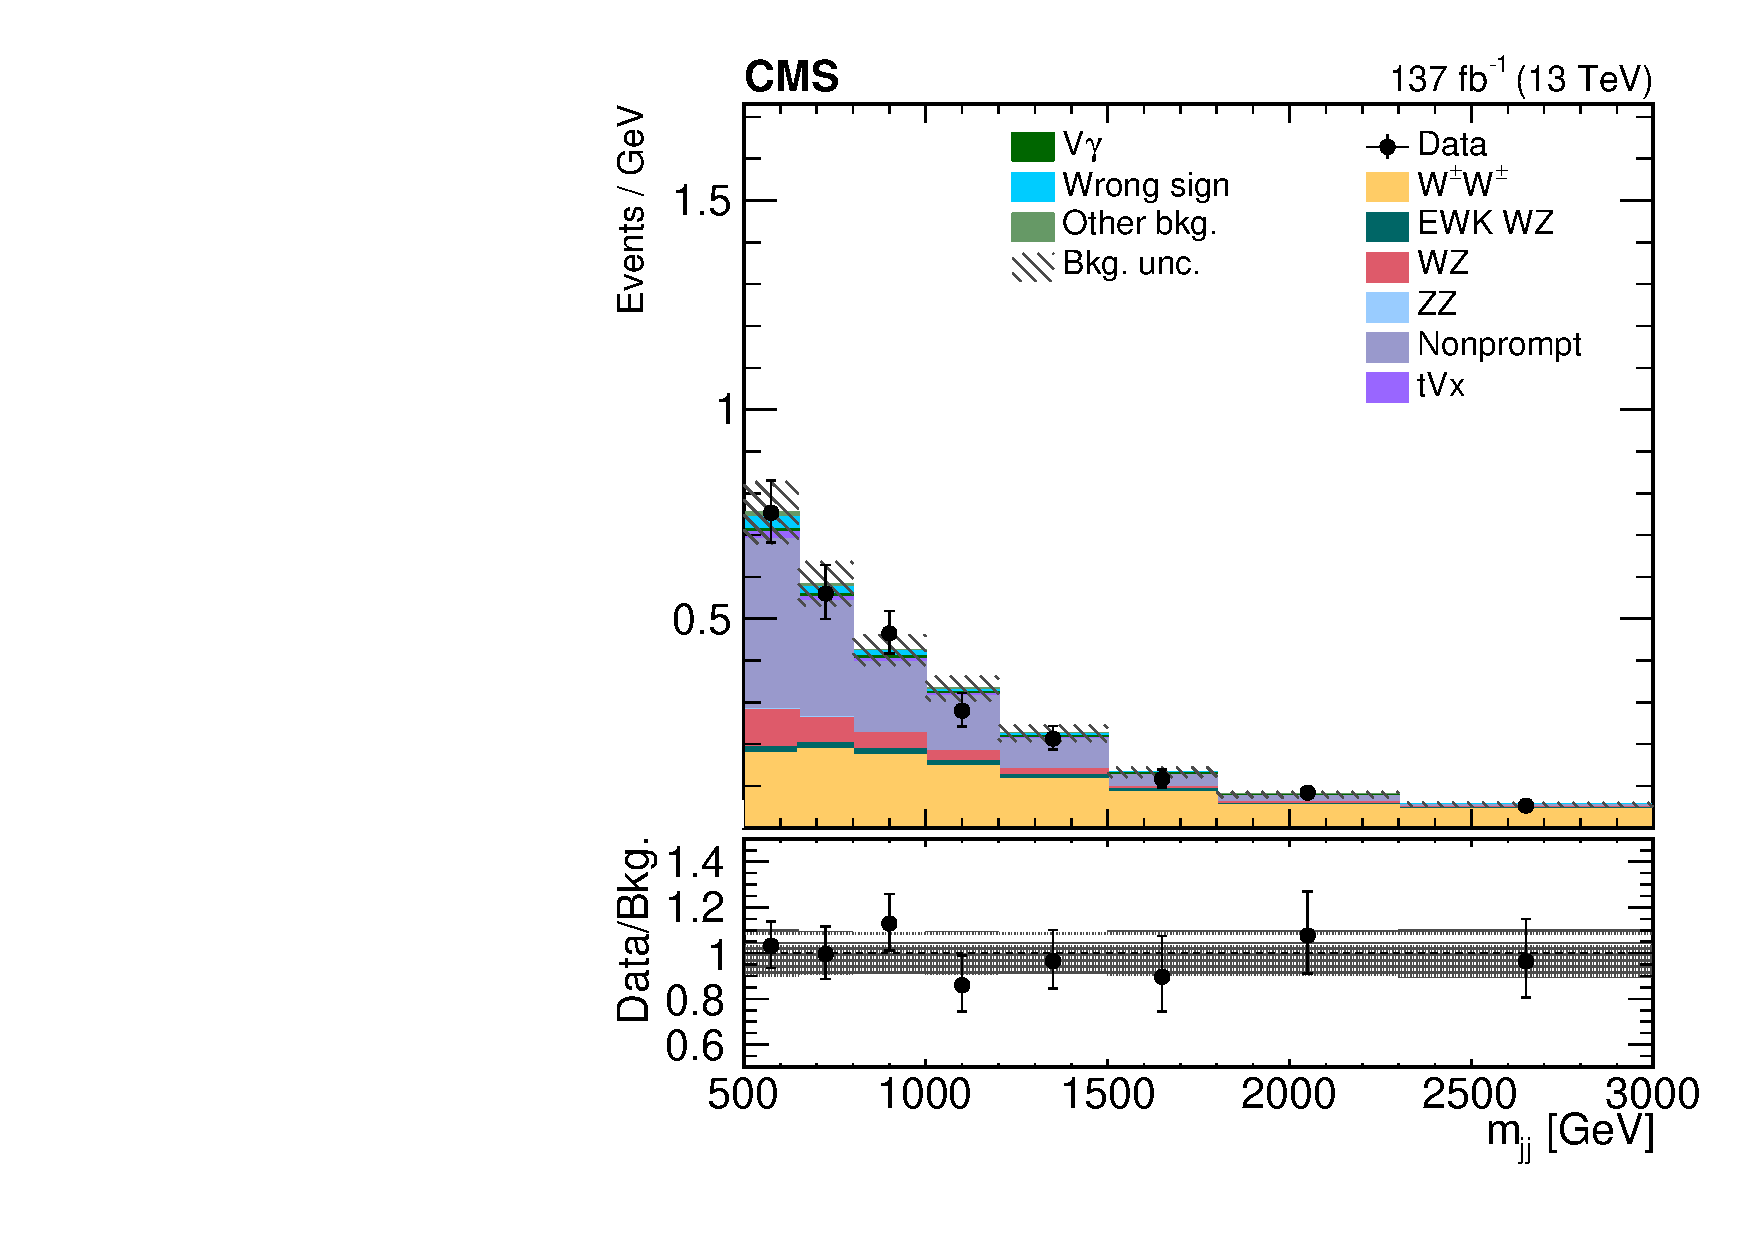
\includegraphics[width=0.49\textwidth]{figures/ssww_wwsel_mjj_2019.pdf}
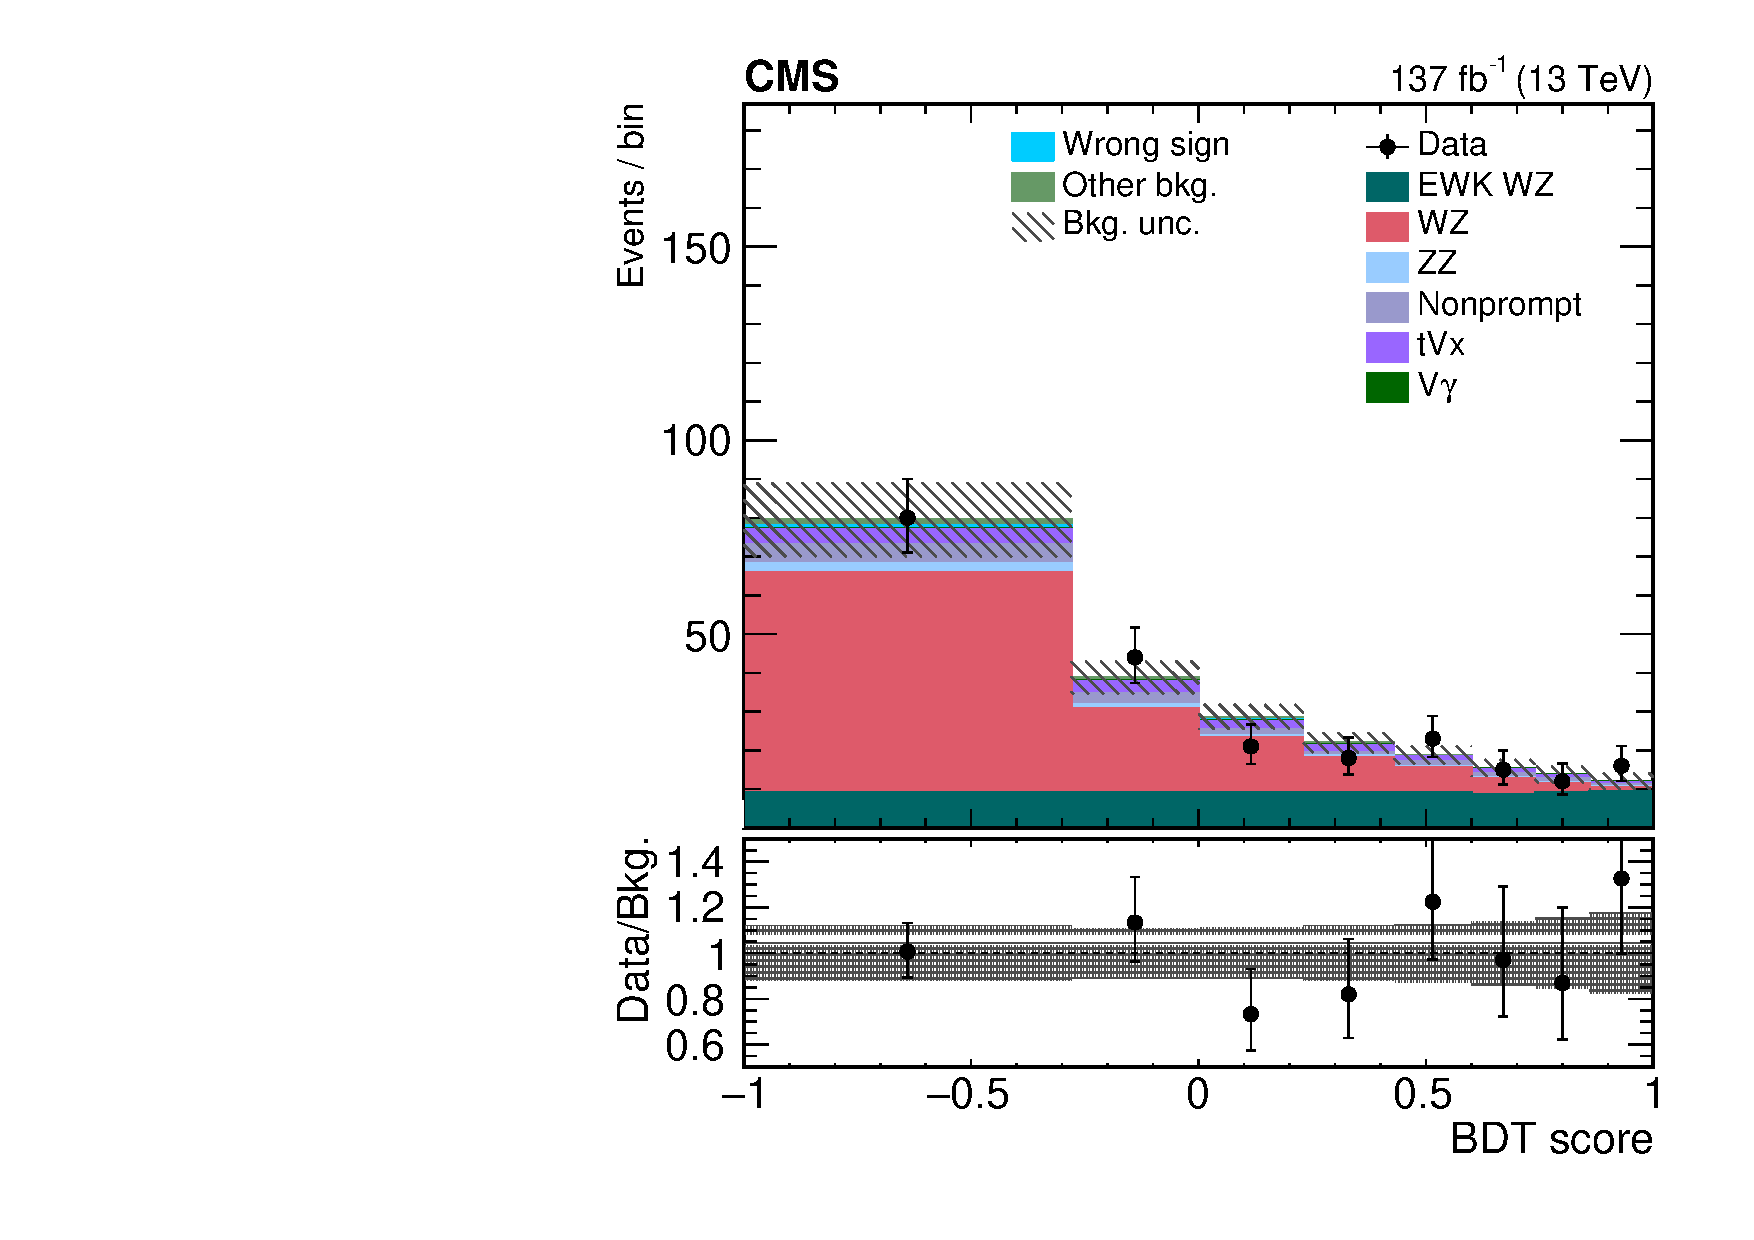
\includegraphics[width=0.49\textwidth]{figures/ssww_wzsel_bdt_2019.pdf}
\caption{Distributions of $\mjj$ in the $\WW$ signal region (left) and  BDT score in the $\WZ$ signal region. The bottom panel in each figure
shows the ratio of the number of events observed in data to that of the total SM prediction. The gray bands represent the uncertainties from the predicted yields.}
\label{fig:signal}
\end{figure*}

\end{document}

